\documentclass[5p]{elsarticle}			% 5p gir 2 kolonner pr side. 1p gir 1 kolonne pr side.
\journal {Veileder}
\usepackage[T1]{fontenc} 				% Vise norske tegn.
%\usepackage[norsk]{babel}				% Tilpasning til norsk.
\usepackage{graphicx}       				% For å inkludere figurer.
\usepackage{amsmath,amssymb} 			% Ekstra matematikkfunksjoner.
%\usepackage{siunitx}					% Må inkluderes for blant annet å få tilgang til kommandoen \SI (korrekte måltall med enheter)
%	\sisetup{exponent-product = \cdot}      	% Prikk som multiplikasjonstegn (i steden for kryss).
% 	\sisetup{output-decimal-marker  =  {,}} 	% Komma som desimalskilletegn (i steden for punktum).
% 	\sisetup{separate-uncertainty = true}   	% Pluss-minus-form på usikkerhet (i steden for parentes). 
\usepackage{booktabs}                     		% For å få tilgang til finere linjer (til bruk i tabeller og slikt).
\usepackage[font=small,labelfont=bf]{caption}	% For justering av figurtekst og tabelltekst.
\usepackage{todonotes}


\makeatletter
\def\ps@pprintTitle{%
  \let\@oddhead\@empty
  \let\@evenhead\@empty
  \let\@oddfoot\@empty
  \let\@evenfoot\@oddfoot
}
\makeatother

\usepackage[utf8]{inputenc}		% gjør slik at vi kan skrive æ,ø,å mm.
\usepackage{parskip}
\usepackage{hyperref}
\usepackage[noabbrev,capitalize]{cleveref}
\usepackage{subcaption}
\usepackage{physics}

% Denne setter navnet på abstract til Sammendrag
\renewenvironment{abstract}{\global\setbox\absbox=\vbox\bgroup
\hsize=\textwidth\def\baselinestretch{1}%
\noindent\unskip\textbf{Abstract}
\par\medskip\noindent\unskip\ignorespaces}
{\egroup}


% Disse kommandoene kan gjøre det enklere for LaTeX å plassere figurer og tabeller der du ønsker.
\setcounter{totalnumber}{5}
\renewcommand{\textfraction}{0.05}
\renewcommand{\topfraction}{0.95}
\renewcommand{\bottomfraction}{0.95}
\renewcommand{\floatpagefraction}{0.35}
\newcommand{\e}{\mathrm{e}}
%%%%%%%%%%%%%%%%%%%%%%%%%%%%%%%%%%%%%%%%%%%%%%%%%%%%%%%%%%%%%%%%%%%%%%%%%
\begin{document}

\begin{frontmatter}
\title{TFY4235 - The World of Quantum Mechanics}

\author[fysikk]{Karl Kristian Ladegård Lockert}
\address[fysikk]{Institutt for fysikk, Norges Teknisk-Naturvitenskapelige Universitet, N-7491 Trondheim, Norway.}
\begin{abstract}
Abstract

\end{abstract}
\end{frontmatter}

\section{Introduction}

\begin{equation}\label{eq:SE}
i\hbar\pdv{\psi}{t} = H\psi
\end{equation}

\begin{equation} 
\label{eq:TISE}
H\psi_n = E_n\psi_n 
\end{equation}
\section{The Hamiltonian}

The Schrödinger equation tells us the time-evolution of the wave function, which, according to the Copenhagen interpretation of quantum mechanics, has the physical interpretation of a probability amplitude when squaring the absolute value. In our current setup, where we have
\begin{equation} 
V = \begin{cases}
0,\quad 0<x<L \\
\infty,\quad \text{otherwise}
\end{cases},
\end{equation}
there is 0\% chance of finding the particle inside the ``walls'' (at $x<0$ or $x> L$). Thus, the wave function must go to zero at these points. Defining $x' = x/L$ and $t'=t/t_0$, and inserting in \cref{eq:SE}.
\begin{align*} 
i\hbar\pdv{\psi}{t} &= i\hbar\pdv{\psi}{t'}\pdv{t'}{t}= \frac{-\hbar^2}{2mL^2}\pdv[2]{\psi}{{x'}}\\
\implies i\pdv{\psi}{t'} &= \frac{-\hbar}{2mL^2 \pdv{t'}{t}}\pdv{\psi}{x'^2}
\end{align*}
Thus, setting
\begin{equation}
t' = \frac{\hbar}{2mL^2}t,\quad x' = \frac{x}{L}
\end{equation}
gives the wanted dimensionless equation
\begin{equation}
\label{eq:SE_dimensionless}
i\pdv{\psi}{t'} = -\pdv[2]{\psi}{{x'}}.
\end{equation}
Inserting our new variables in \cref{eq:TISE} with \[H = \frac{\hat p^2}{2m} + V(x) =  -\frac{-\hbar}{2mL^2} \pdv[2]{{x'}} + \tilde{V}(x'),\] we get
\begin{align} 
\frac{-\hbar^2}{2mL^2}\pdv[2]{\psi_n}{{x'}} &= E_n\psi_n \implies \nonumber\\
\label{eq:eig}
-\pdv[2]{\psi_n}{{x'}} &= \lambda_n\psi_n,
\end{align}
with the relation 
\begin{equation} 
\lambda_n = \frac{2mL^2 E_n}{\hbar^2}
\end{equation}
between the energy levels and the dimensionless eigenvalues. The boundary conditions that the wave function disappears in the walls, but the walls are now at $x' = 0$ and $x' = 1$. It is now clear that choosing $x_0 = L$ is suitable, as it makes us able to work on the simple domain $[0,1]$. Any other proportionality constant $\alpha\in \mathbb{R}$ such that $x' = \alpha x/ L$ should work as well, scaling both the time and energies by a factor $\alpha^2 $, as long as $x'$ is dimensionless. Other scaling possibilities are also possible, and have consequences for the analytic expressions for $\psi$. For example scaling the interval to be mirrored about $x = 0$ would only pick out the even terms in a Fourier series expansion.

Solving \cref{eq:eig} with the imposed boundary conditions can be done analytically in the following manner.
Since we are looking for solutions that have self-similar second derivatives with an extra minussign, we guess a solution on the form 
$\psi = A_n\sin(\sqrt{\lambda_n}x') + B_n\cos(\sqrt{\lambda_n}x')$. The boundary condition $\psi(x'=0) = 0$ gives $B_n = 0$, while the boundary condition $\psi(x'=1) = 0$ gives the restriction to $\lambda_n$ that $\sqrt{\lambda_n} = n\pi$, hence the labels $n$ are also justified. Our analytic solution is therefore 
\begin{equation}
\psi_n(x') = \mathcal{N}\sin(\pi n x'),
\end{equation} 
where $\mathcal{N}$ is a normalization constant to be decided.
\begin{align*} 
1 &= \braket{\psi_n}{\psi_n} = \mathcal{N}^2\int_{0}^{1}\dd{x'}\sin[2](n\pi x') \\
&=\mathcal{N}^2\int_0^1\dd{x'}\frac{1-\cos(2\pi n x')}{2}
= \frac{\mathcal{N}^2}{2} \\
&\implies \mathcal{N} = \sqrt{2},
\end{align*}
and we have the analytic solution as announced in \cite{assignment}.

The implementation of a finite-difference-scheme is done using sparse matrix formatting for the cases when the discretization step is very small. Otherwise a dense matrix format is sufficient.
\todo{Sett inn graf av egenverdier sammenliknet med analytisk uttrykk.}


The implementation of 
\begin{equation} 
\alpha_n = \braket{\psi_n}{\Psi_0} = \int\dd{x'}\psi_n^*(x')\Psi_0(x')
\end{equation}
can be done in a simple fashion by taking optimized inner-product implementations for general vectors, so calculating the actual integral is actually not needed. \todo{Finn ut om simpsons metode funke greit, og eventuelt sammenlikn.}


\todo{Scaling of error }
To compute the error of a numerical solution, we must have a metric of some sort. Let us use 
\begin{equation} 
E[\bar\psi_n(x')] = \int\dd{x'}|\bar \psi_n(x')-\psi_n(x')|^2
\end{equation}
as an example, where the bar denotes the numerical approximation to the analytic function.
Using the reduced units previously discussed, we can express the full state
\begin{equation} 
\Psi(x, t) = \sum_n\alpha_n\exp(-\frac{iE_n t}{\hbar})\psi_n(x)
\end{equation}
as
\begin{align*} 
\sum_n\alpha_n\exp(-\frac{iE_n t}{\hbar})&\psi_n(x) =\sum_n\alpha_n\exp(-\frac{iE_n t}{\hbar})\psi_n(x) \\ &=\sum_n\exp(-\frac{i\frac{\hbar^2\lambda_n}{2mL^2}\frac{2mL^2t'}{\hbar}}{\hbar})\psi_n(x') \\&= \sum_n\alpha_n\exp(-i\lambda_n t')\psi_n(x').
\end{align*}

\section{Adding a barrier to the box-potential}
Let us now consider a potential barrier in the box, modeled by the dimensionless potential $\nu(x') = t_0V_0/\hbar$, where $t_0 =\frac{2mL^2}{\hbar}$ as in \cref{eq:normalized_stuff}, and is given by
\begin{equation} 
\nu(x') = \begin{cases}
0,\quad &0<x'<\frac{1}{3} \\
\nu_0 = \frac{2mL^2V_0}{\hbar^2},\quad &\frac{1}{3}<x'<\frac{2}{3} \\
0,\quad &\frac{2}{3}<x'<1 \\
\infty ,\quad &\text{otherwise}
\end{cases}
\end{equation}
Thus, setting $\nu_0$ to 0 is the same task as we had for the previous case, since we have the same boundary conditions and a vanishing potential between the edges, which ensures that the matrix-representation (and thus the eigenvalues) of the operator acting on the wave function is equal. 
Now we set $\nu_0 = 10^3$.
Comparing the energy eigenvalues for the problem, we find that some seem to be equal, i.e. there seems to be degeneracy in the system. This cannot be, since we are in 1D with a discrete energy spectrum \cite{hemmer1985kvantemekanikk}. Indeed, the states are equal, as we can see for the lowest lying energy eigenfunctions in \cref{fig:degeneracy}.
\begin{figure}
	\centering
	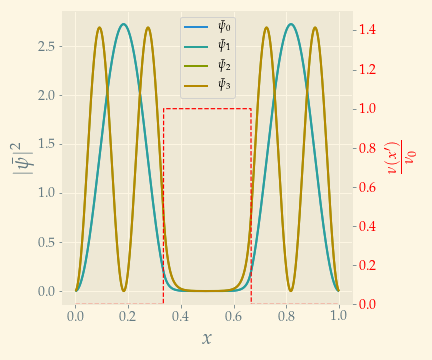
\includegraphics[width=\linewidth]{img/degeneracy.png}
	\caption{Degeneracy of the ground state and first excited states plotted together with the potential.}
	\label{fig:degeneracy}
\end{figure}
We now prepare the initial state 
\begin{equation} 
\label{eq:psi0}
\Psi_0 = \frac{1}{\sqrt{2}}\left( \psi_1(x') + \psi_2(x') \right)
\end{equation}
and let it evolve from $t_0'=0$ to \begin{equation}
\label{eq:time}
t_1'=\frac{\pi}{\lambda_2 -\lambda_1},
\end{equation}we find that the particle has tunneled from one side of the barrier to the other! This is shown in \cref{fig:tunneling}. 
\begin{figure}
	\centering
	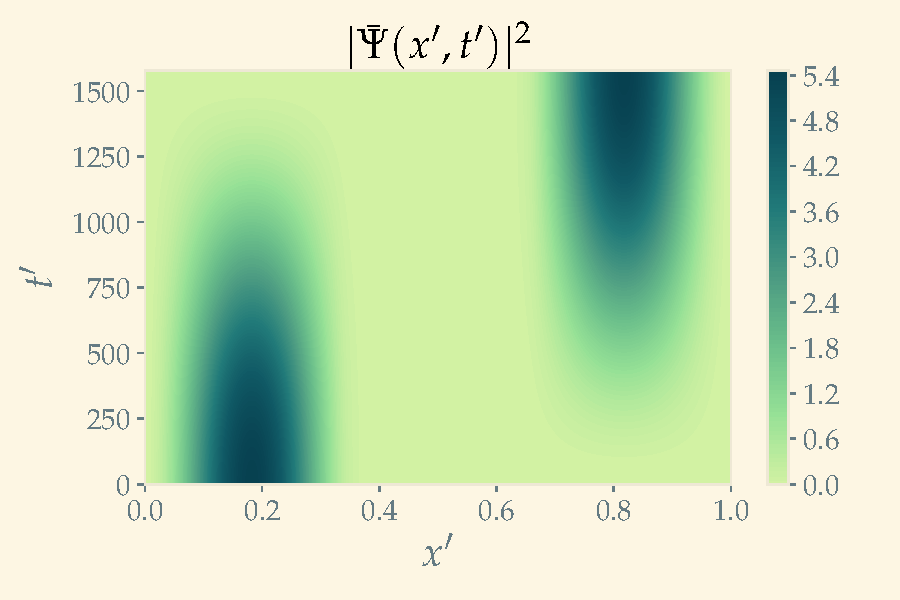
\includegraphics[width=\linewidth]{img/tunneling.pdf}
	\caption{Tunneling across the potential barrier.}
	\label{fig:tunneling}
\end{figure}
We can see that the initial state (on the left side of the potential barrier) ``leaks'' into the opposite side as time progress. Inserting \cref{eq:time} into \cref{eq:full_state}, we find (after some manipulation) 
\begin{equation} 
\Psi(x', t'_1) = C\left(\psi_2(x')-\psi_1(x')\right)
\end{equation}
for a normalization constant $C$. 
This is the initial state mirrored about $x' = 1/2$.

\section{Root finding}

Following ref. \cite{assignment}, the eigenvalues of the analytic solutions are given by the roots of the function $f(\lambda)$, shown in \cref{fig:f}. 
\begin{figure}
	\centering
	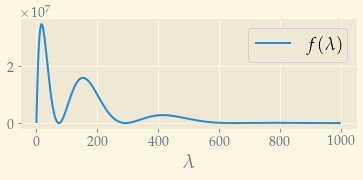
\includegraphics[width=\linewidth]{img/f}
	\caption{The analytic expression for finding the eigenvalues. }
	\label{fig:f}
\end{figure}
This is in good agreement with the computed eigenvalues. By using SciPy's \cite{2020SciPy-NMeth} optimized root-finding algorithm with the computed eigenvalues as the initial guess, we find three distinct eigenvalues below $\nu_0 = 10^3$.
Using the implementation of the root finder, the roots of $f(\lambda)$

\begin{table}
	\centering
\begin{tabular}{|c|c|}
	\hline
Computed $\bar\lambda$ & Roots of $f(\lambda) $\\
	\hline 
	73.49662578 & 73.93560016 \\ 

	73.49861656 &  \\ 

	291.77230762 & 293.49231502 \\ 
 
	291.79660664 &  \\ 
 
	644.62162712 & 648.26437316 \\ 

	645.10279446 &  \\
	\hline
\end{tabular}
	\caption{A comparison of computed eigenvalues and computed roots of the analytic expression for $f(\lambda)$. The units are given by \cref{eq:energy_conversion}. }
\end{table}

\bibliographystyle{unsrt}
\bibliography{bib}

\end{document}
